\documentclass{article}

\usepackage{graphicx}

\begin{document}

\title{Homework4}
\author{Qi Mao\\
  \texttt{maoxx241@umn.edu}}
\maketitle
\section{Question1:}
[20 points] For each of the following sentences, decide if the logic sentence given is a correct translation of the English sentence or not. If not explain briefly why not and correct it:
\begin{itemize}
    \item 1.	All houses have at least one bathroom. \newline
    $\forall$ x [House(x) $\wedge$ $\exists$ y Bathroom(y)] $\Rightarrow$ In(x,y)\newline
    \break
    Incorrect. This sentence means there is a Bathroom in every house. This should be:\newline
    $\forall$x house(x) $\Rightarrow$ $\exists$y bathroom(y) $\wedge$ In(y, x)

    \item 2.    There is a house in Minneapolis which costs more than any other house. \newline
    $\forall$ x [House(x) $\wedge$ In(x,Minneapolis)] $\Rightarrow$ [$\exists$ y House(y) $\wedge$ Cost(y) $>$ Cost(x)]\newline
    \break
    Incorrect. This sentence means any houses in Minneapolis, there is house cost more than it. This should be:\newline
    $\exists$y house(y) $\wedge$ In(y, Minneapolis) $\wedge$ [$\forall$x house(x) $\Rightarrow$ cost(y)$>$cost(x) $\wedge$ x$\neq$y]

    \item 3.    There is only one house in Minneapolis that is pink. \newline
    $\exists$ x House(x) $\wedge$ In(x,Minneapolis) $\wedge$ Color(x,Pink)\newline
    \break
    Incorrect. It doesn’t show that there is only one. This should be:\newline
    $\exists$ x House(x) $\wedge$ In(x,Minneapolis) $\wedge$ Color(x,Pink) $\wedge$ $\forall$y [house(y) $\wedge$ in(y, Minneapolis) $\wedge$ Color(y,Pink) $\Rightarrow$ x=y]

    \item 4.    Some houses cost less than some apartments. \newline
    $\exists$ x House(x) $\wedge$ $\exists$ y Apartment(y) $\Rightarrow$ Cheaper(x,y)\newline
    \break
    Incorrect. $\Rightarrow$should be $\wedge$. This should be:\newline
    $\exists$ x House(x) $\wedge$ $\exists$ y Apartment(y) $\wedge$ Cheaper(x,y)
    \item 5.    There are fastfood places in every city. \newline
    $\forall$ x $\forall$ y [City(x) $\wedge$ Fastfood (y)] $\Rightarrow$ In(y,x)\newline
    \break
    Incorrect. It means all fastfood places in all cities. This is also incorrect.
    This should be:\newline
    $\exists$ x Fastfood(x) $\wedge$ $\forall$ y City(y) $\Rightarrow$ In(x,y)

\end{itemize}

\section{Question2}
[20 points] Convert these English sentences to predicate calculus, using the following predicates: Cat(x) = x is a cat; Bird(x) = x is a bird; Dog(x) = x is a dog; Animal(x) = x is an animal; Person(x) = x is a person. Owns(x,y) = x owns y; Likes(x,y) = x likes y, Kill(x,y) = x kills y. John is a constant.
\begin{itemize}
    
\item 1.    Birds do not like cats.\newline
$\forall$ x,y Bird(x) $\wedge$ Cat(y) $\Rightarrow$$\neg$Likes(x,y)
\item 2.    Any person who owns a cat does not own a bird.\newline
$\forall$ x[ Person(x) $\wedge$ $\exists$y Cat(y) $\wedge$ Owns(x,y) ] $\Rightarrow$ $\neg$[$\exists$z Bird(z) $\wedge$ Owns(x,z)]
\item 3.    No person would kill a cat.\newline
$\neg$[$\exists$ x Person(x)$\wedge$ $\exists$y Cat(y) $\wedge$ Kill(x,y)]
\item 4.    Some persons own a cat and a dog.\newline
$\exists$ x Person(x) $\wedge$ $\exists$y Cat(y) $\wedge$ Owns(x,y) $\wedge$ $\exists$z Dog(z) $\wedge$ Owns(x,z)
\item 5.    John owns only one bird.\newline
$\exists$ x Bird(x) $\wedge$ Owns(John,x) $\wedge$ $\forall$y [Bird(y) $\wedge$ Owns(John, y)  $\Rightarrow$ x=y]
\end{itemize}

\section{Question3}
[10 points]
\begin{itemize}
    
\item 1.    Write the knowledge given below in predicate calculus using the following predicates: Person(x) = x is a person; Rich(x) = x is rich; Happy(x) = x is happy; Read(x) = x can read; Exciting(x) = x has an exciting life; Stupid(x) = x is stupid 
The change made to Exciting is to make things easier. You are free to use the predicates I had before \newline
"All persons who are rich and are not stupid are happy. Persons who can read are not stupid. Happy persons have exciting lives. John is a person. John can read and he is rich. "
\begin{itemize}
    \item All persons who are rich and are not stupid are happy.\newline
    $\forall$x[Person(x) $\wedge$Rich(x) $\wedge$$\neg$Stupid(x)] $\Rightarrow$Happy(x)
    \item Persons who can read are not stupid.\newline
    $\forall$x [Person(x) $\wedge$ Read(x)]$\Rightarrow$$\neg$Stupid (x)
    \item Happy persons have exciting lives.\newline
    $\forall$x [Person(x) $\wedge$ Happy(x)] $\Rightarrow$Exciting(x)
    \item John is a person.\newline
    Person(John)
    \item John can read and he is rich.\newline
    Read(John) $\wedge$Rich(John)
\end{itemize}
\item 2.    convert to CNF\newline
1.	$\neg$ Person(x) $\vee$ $\neg$Rich(x) $\vee$ Stupid(x) $\vee$ Happy(x)\newline
2.	$\neg$ Person(x) $\vee$ $\neg$Read(x) $\vee$$\neg$Stupid (x)\newline
3.	$\neg$Person(x) $\vee$ $\neg$Happy(x) $\vee$Exciting(x)\newline
4.	Person(John)\newline
5.	Read(John)\newline
6.	Rich(John)

\item 3.    Answer the question "is there anyone who has an exciting life?" Notice that this is a question that requires not just True or False as an answer.
\break
Yes. Because John can read, and John is rich. so John is not stupid.Person who is rich and not stupid is happy and person who is happy has an exciting life.
\end{itemize}

\section{Question4}
[20 points] Prove by resolution that the following set of clauses (in predicate calculus) is unsatisfiable. Assume that upper case arguments are constant, lower case arguments are variable:
\begin{itemize}
    
\item 1.    G(B)
\item 2.    $\neg$ G(x) $\vee$ H(x)
\item 3.    $\neg$ H(z) $\vee$ I(z)
\item 4.    $\neg$ H(w) $\vee$ J(w,D)
\item 5.    $\neg$ I(B) $\vee$ J(C,B)
\item 6.    $\neg$ I(q) $\vee$ $\neg$ J(q,y)
\begin{center}
    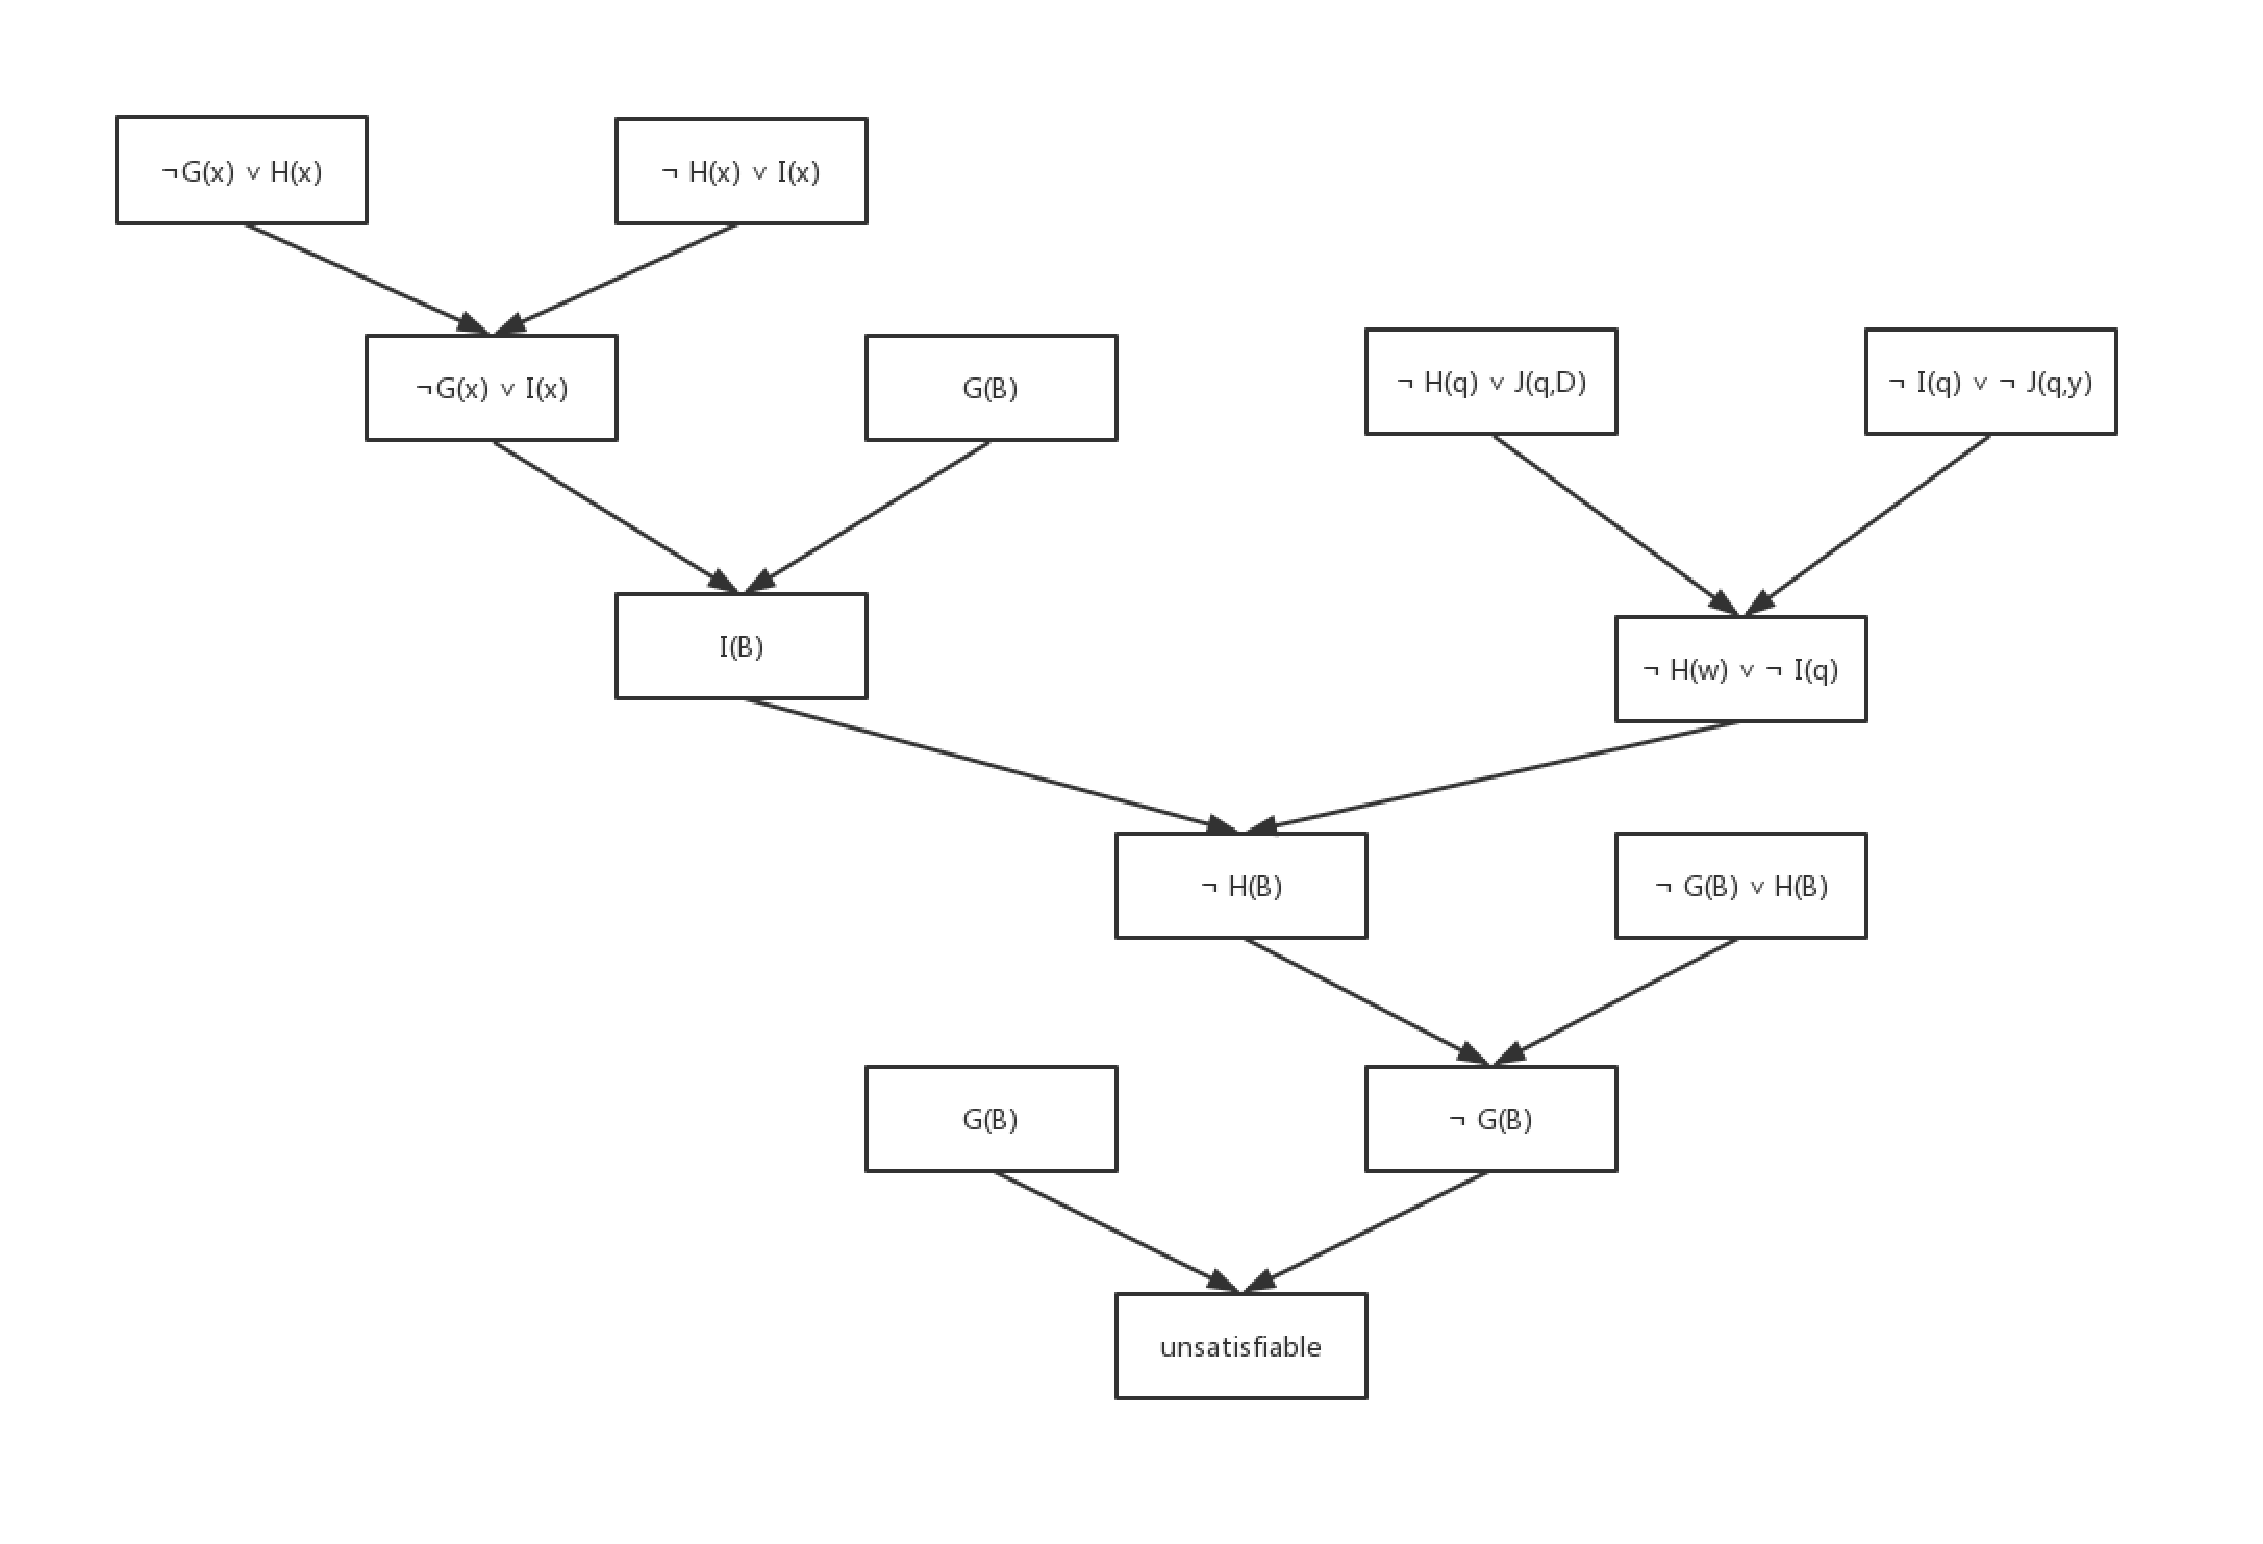
\includegraphics[scale=0.4]{pic}
\end{center}
\end{itemize}

\section{Question5}
[30 points]
\begin{itemize}
    
\item 1.    Write the following statements in predicate calculus:
        \begin{itemize}
            \item A truck is a vehicle.\newline
            $\vee$x Truck(x) $\Rightarrow$ Vehicle(x)
            \item A SUV is a vehicle.\newline
            $\vee$x SUV(x) $\Rightarrow$ Vehicle(x)
            \item A car is a vehicle.\newline
            $\vee$x Car(x) $\Rightarrow$ Vehicle(x)
            \item A truck is bigger than a SUV.\newline
            $\vee$x Truck(x) $\wedge$ $\vee$y SUV(y)$\Rightarrow$ Big(x , y)
            \item There is a SUV that is bigger than every car.\newline
            $\exists$x SUV(x) $\wedge$ $\vee$y Car(y) $\Rightarrow$ Big(x , y)
            \item A RAM is a truck.\newline
            Truck(RAM)
            \item A Tesla is a car.\newline
            Car(Tesla)
            \item Bigger is transitive, i.e. if x is bigger than y and y is bigger than z then x is bigger than z.
            $\vee$x , y , z Big(x,y) $\wedge$Big(y,z) $\Rightarrow$Big(x,z)
        \end{itemize}
\item 2.    Convert them to CNF. Pay attention to how you skolemize existentially quantified variables. Recall that a Skolem constant cannot be unified with another constant except itself, but it can be unified with a variable.
\begin{itemize}
    \item 1.	$\neg$Truck(x) $\vee$ Vehicle(x)
    \item 2.	$\neg$SUV(x) $\vee$ Vehicle(x)
    \item 3.	$\neg$Car(x) $\vee$ Vehicle(x)
    \item 4.	$\neg$Truck(x) $\vee$$\neg$SUV(y) $\vee$ Big(x , y)
    \item 5.	$\neg$SUV(x) $\vee$ $\neg$Car(y) $\vee$ Big(x , y)
    \item 6.	Truck(RAM)
    \item 7.	Car(Tesla)
    \item 8.	$\neg$Big(x,y) $\vee$$\neg$Big(y,z) $\vee$Big(x,z)
\end{itemize}
\item 3.    Prove by resolution with refutation: "A RAM is bigger than a Tesla". Remember that a Skolem constant cannot be unified with another constant except itself, but it can be unified with a variable.
\begin{itemize}
    \item 1.	$\neg$Truck(x) $\vee$ Vehicle(x)
    \item 2.	$\neg$SUV(x) $\vee$ Vehicle(x)
    \item 3.	$\neg$ Car(x) $\vee$ Vehicle(x)
    \item 4.	$\neg$Truck(x) $\vee$ $\neg$SUV(y) $\vee$ Big(x, y)
    \item 5.	Truck(RAM)
    \item 6.	Car(Tesla)
    \item 7.	$\neg$ Big(x,y) $\vee$ $\neg$ Big(y,z) $\vee$ Big(x, z)
    \item 8.	$\neg$Big(Truck(RAM), Car(Tesla))
\end{itemize}
\end{itemize}
\end{document}